\chapter{Methodology}%
\label{chapter:methodology}

As defined earlier in section~\ref{section:Goals}, the primary goal of this dissertation is to leverage the Human-Robot Collaboration \ac{HRC} paradigm by integrating \ac{MR} technologies alongside robot capabilities to enhance remote collaboration. In order to achieve this, a conceptual model is further implemented.

\section{Conceptual Model}
In order to start addressing the mentioned challenges, a first effort has been made. A robotic arm from Universal Robots, UR10e, shown in the figure \ref{f:ur10e_iris}, available at IRIS LAB, was used as a dynamic agent to assist in shared activities.
%  add a footnote to the robot model in universal robots website

\begin{figure}[h]
    \centering
    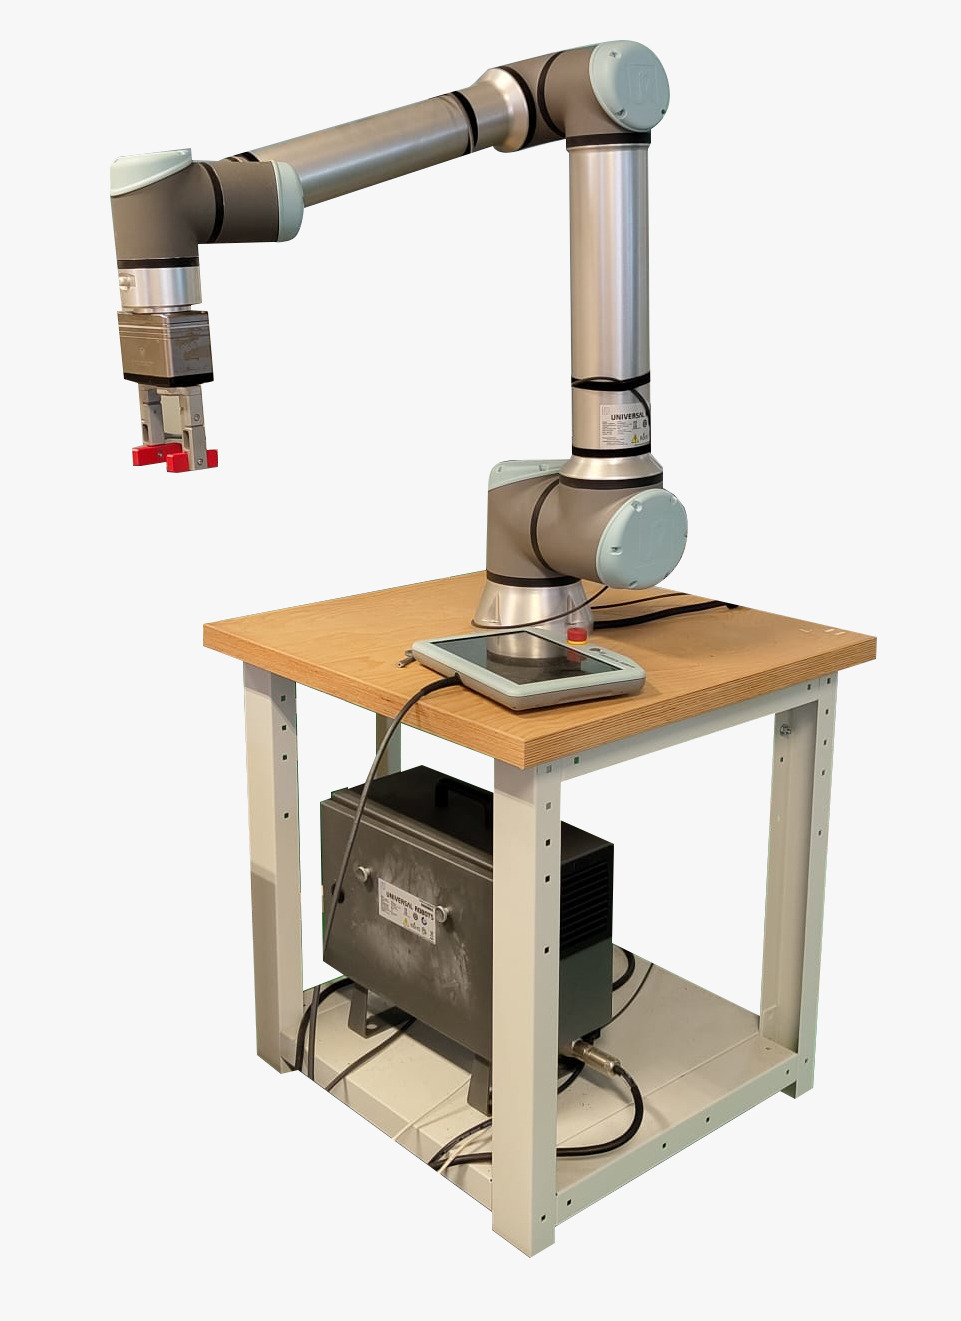
\includegraphics[width=0.4\linewidth]{figs/ur10e.jpeg}
    \caption{Robot UR10e used for the development of the dissertation work, available at IRIS-LAB, University of Aveiro}
    \label{f:ur10e_iris}
\end{figure}

Afterwards, the framework required to integrate the \ac{MR} technologies with the robotic arm was thoroughly discussed with the supervisors, leading to the following components:
\begin{itemize}
    \item \textbf{On-Site Interaction:}
    \begin{itemize}
        \item Implement an UR10e digital model into the Unity 3D simulation environment
        \item Utilize marker detection, utilizing Vuforia, to align the digital model with the physical robot
        \item Perform pose registration to ensure accurate spatial alignment between the virtual and physical models
        \item Develop a user-friendly interface for robot manipulation using \ac{HHDs}
        \item Implement visual and audio cues for user awareness and accident prevention 
    \end{itemize}
    \item \textbf{Remote Visualization and Interaction:}
    \begin{itemize}
        \item Enable bilateral communication between the robot and the Unity digital twin
        \item Provide remote participants with a foundational 2D interface, such as a laptop screen, to visualize the collaboration scenario and 
        task context.
        \item Implement real-time updates of the robot's position and workspace visualization
        \item Develop the capability for remote operation of the robot via the \ac{MR} application, enhancing the remote participant's ability to 
        interact and manipulate the collaborative environment.
    \end{itemize}
    \item \textbf{Automation and Immersion:}
    \begin{itemize}
        \item Integrate a camera into the robot and develop a camera feed transmission to provide real-time updates of the robot's position and workspace visualization
        \item Share this information with remote participants, assisting on-site participants by delegating visual sharing to the robot.
    \end{itemize}
\end{itemize}



\section{Digital Model Implementation of the Robot}
\label{section:digital-model}

\subsection{Unity}



Unity is a dynamic and versatile game engine developed by Unity Technologies \footnote{Unity Technologies \url{https://unity.com/} Accessed: 2024-09-30}, widely recognized for revolutionizing game development over the past few years. Beyond gaming, it has become a prominent tool for creating \ac{AR}, \ac {VR}, and \ac{MR} applications. Its user-friendly interface empowers developers to rapidly craft immersive experiences while simplifying complex development processes.

By offering an \ac{IDE} that combines \ac{GUI} manipulation of scene objects with a code editor, similar to Visual Studio, it allows developers to build virtual scenes by either creating or integrating 2D and 3D assets as well as apply attributes such as lighting, audio, physics properties, animations, and interactive gameplay logic. Afterwards, these composed scenes come to life, rendering them in real-time at frame rates that create smooth motion and immersive experiences.

One of Unity's significant advantages is its extensive platform compatibility. It supports development for various operating systems, including Windows, and Linux, as well as mobile platforms like iOS and Android. Additionally, a wide range of devices spanning \ac{AR},\ac{VR},\ac{MR} technologies are supported.

Unity's choice for developing the \ac{MR} application was advised by both supervisors regarding its versatility as well as its robust capabilities and extensive feature set.

\subsection{Digital Robot Model - URDF Importer Package}
% % % foi necessário encontrar um modelo do robot a ser utilizado - UR10e que se encontra no IRIS lab
% To successfully develop the XR application for controlling the UR10e robot, it was essential to identify a model that closely mirrors 
% the actual robot. The Unity Robotics Hub \footnote{Unity Technologies \url{https://github.com/Unity-Technologies/Unity-Robotics-Hub} 
% Accessed: 2024-02-02} facilitates the integration of robotics into Unity projects via the URDF-Importer package 
% \footnote{Unity Technologies \url{https://github.com/Unity-Technologies/URDF-Importer} Accessed: 2024-02-02}. 
% However, challenges arose when attempting to import the UR10e \textit{.urdf} model into the Unity environment. To overcome this, 
% a UR10 model, sourced from a GitHub repository \footnote{PositronicsLab \url{https://github.com/PositronicsLab/reveal_packages/tree/master/industrial_arm/scenario/models/urdf/ur10} Accessed: 2024-02-05} 
% was used, due to its resemblance to the UR10e robot. This was discussed with the educators overseeing the dissertation development, 
% and it was agreed that this approach would not pose any issues.

% In the figure \ref{f:ur10_marker_unity} it is possible to see the digital UR10 model positioned related to the aruco marker 
% (\ref{f:aruco_marker}), in a simulated Unity environment.
% \begin{figure}[h]
% \centering
% 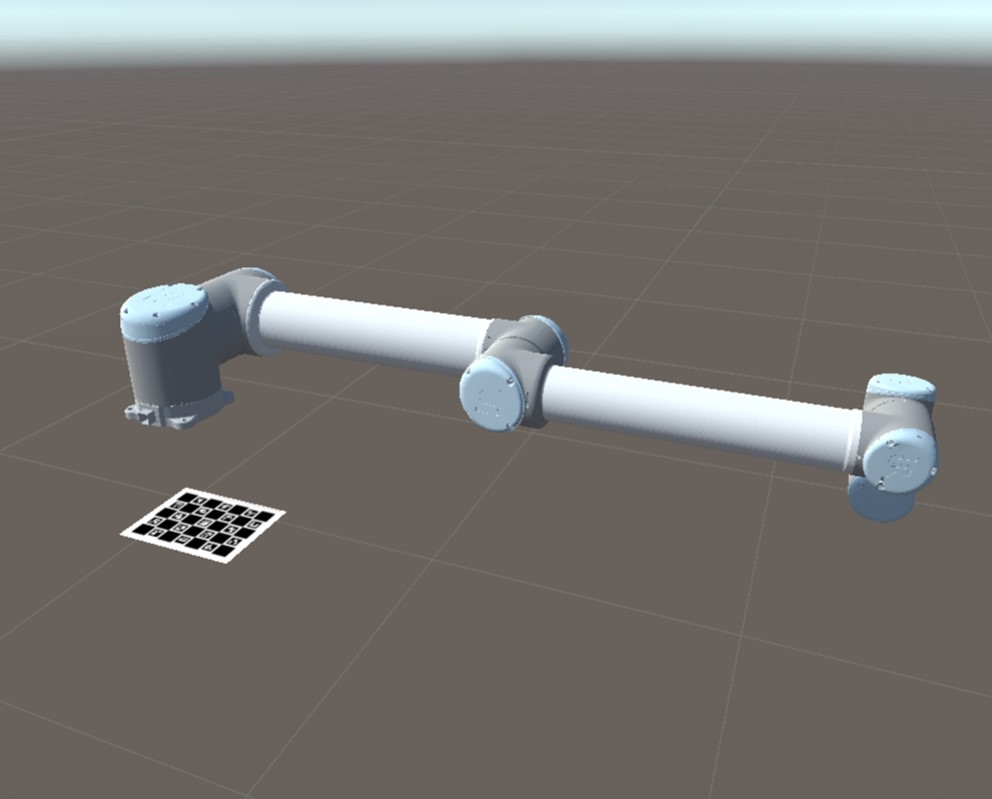
\includegraphics[width=0.6\textwidth]{figs/robot_marker_unity.jpg}
% \caption{Digital UR10 model related to the aruco marker, on Unity environment}
% \label{f:ur10_marker_unity}
% \end{figure}
 - commented this part because text is below - choose whether to use this or the text below

    % foi necessário encontrar um modelo do robot a ser utilizado - UR10e que se encontra no IRIS lab
    To successfully develop the \ac{MR} application for controlling the UR10e robot, it was essential to identify a model that closely mirrors 
    the actual robot. The Unity Robotics Hub \footnote{Unity Robotics Hub \url{https://github.com/Unity-Technologies/Unity-Robotics-Hub} 
    Accessed: 2024-02-02} facilitates the integration of robotics into Unity projects via the URDF-Importer package 
    \footnote{Unity URDF Importer \url{https://github.com/Unity-Technologies/URDF-Importer} Accessed: 2024-02-02}. 
    
    However, instead of importing the UR10e \textit{.urdf} model into the Unity environment, a UR10 model, sourced from a GitHub repository \footnote{PositronicsLab \url{https://github.com/PositronicsLab/reveal_packages/tree/master/industrial_arm/scenario/models/urdf/ur10} Accessed: 2024-02-05} 
    was used, due to its resemblance to the UR10e robot. 
    % This was discussed with the educators overseeing the dissertation development, and it was agreed that this approach would not pose any issues.


% \ac{MR} alongside a static robotic arm (UR10e) to support remote collaboration scenarios. This involves transforming human-robotic collaboration by integrating \ac{MR} technologies and robotic capabilities to enhance both on-site and remote collaboration experiences.

% Unity 3D engine will allow robot model development, enabling detailed and interactive digital twins with bilateral communication capabilities. By utilizing Vuforia for precise pose registration, the system ensures accurate spatial alignment between the virtual and physical robots.

% To enhance user awareness and prevent accidents, the system will implement visual and audio cues within the \ac{AR} environment, including safety-zone interactions and audio alerts. These features provide intuitive feedback to users, improving situational awareness during human--robot collaboration. The robot manipulation interface will be designed to be user-friendly, allowing non-expert users to operate the robot remotely using a handheld device (\ac{HHD}). This accessibility ensures that a wider range of users can effectively interact with the robotic system without extensive training.

% Real-time updates of the robot's position and workspace visualization will be provided through camera feed transmission, offering remote users a comprehensive view of the operational environment. This feature addresses the limitations identified in existing literature, where remote users often lack sufficient context and visibility of the workspace.

% % Furthermore, the proposed system will address challenges identified in the state-of-the-art review, such as networking latency and positioning accuracy. By implementing optimized communication protocols and advanced tracking algorithms, the system aims to ensure efficient and safe human--robot collaboration. These improvements will not only enhance the performance of the system but also contribute valuable insights to the field, bridging the gap between on-site and remote interaction capabilities in industrial applications.

% Overall, this project seeks to expand upon current research by providing a holistic solution that integrates advanced technologies to facilitate seamless collaboration between humans and robots, regardless of physical location. By focusing on both on-site and remote users, the system aims to enhance flexibility, safety, and efficiency in various industrial scenarios.

\section{Pose registration}

After having successfully imported the \ac{URDF} model of the real robot into the Unity environment, the next step was to ensure that the digital model was accurately aligned with the physical robot. 

\subsection{Vuforia}
\label{section:marker-detection}
% 
% Vuforia is a software platform that enables the creation of \ac{ar} experiences. 
% % Integrated with Unity, a leading platform for developing games and interactive applications, Vuforia simplifies the incorporation 
% of AR into mobile and digital apps. 
% It uses computer vision technologies to recognize and track images and objects in the real world, allowing developers to overlay digital 
% content precisely.

% The marker illustrated in Figure \ref{f:aruco_marker} was selected following initial attempts that yielded inconsistent results when using 
% the laptop's camera, shown in the figure \ref{fig:camera-c922}, to scan the environment. This particular marker demonstrated greater stability, 
% enabling the precise positioning of the digital UR10 model in alignment with the physical surroundings. Consequently, this facilitated the accurate 
% overlay of the digital UR10 model onto the actual UR10e robot, enhancing the integration of virtual and real-world elements.

% \begin{figure}[h]
%     \centering
%       \begin{subfigure}[b]{0.45\textwidth}
%       \centering
%       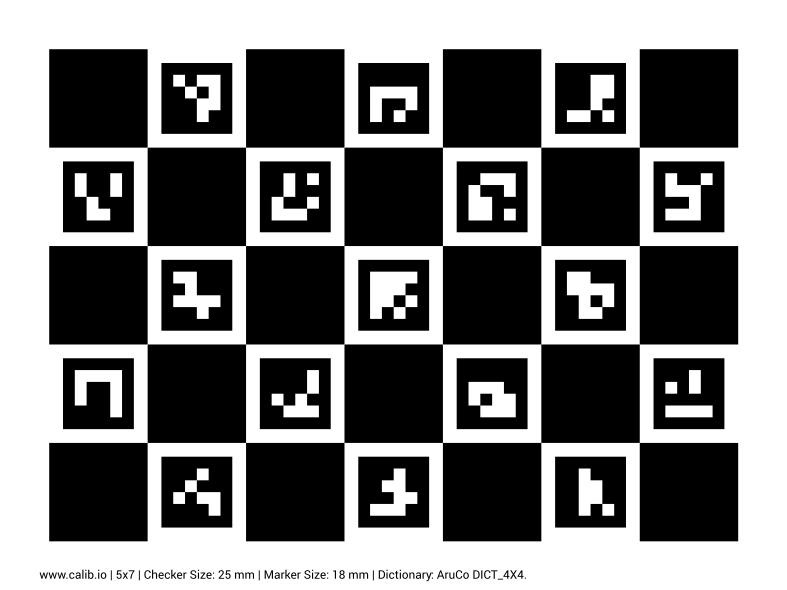
\includegraphics[width=0.7\textwidth]{figs/calib_io_charuco_200x150_5x7_25_18_DICT_4X4.png}
%       \caption{ArUco marker used to allow the segmentation for aligning the digital twin accordingly to the real environment}
%       \label{f:aruco_marker}
%       \end{subfigure}
%         \hfill % This command adds space between the subfigures
%       \begin{subfigure}[b]{0.45\textwidth}
%           \centering
%           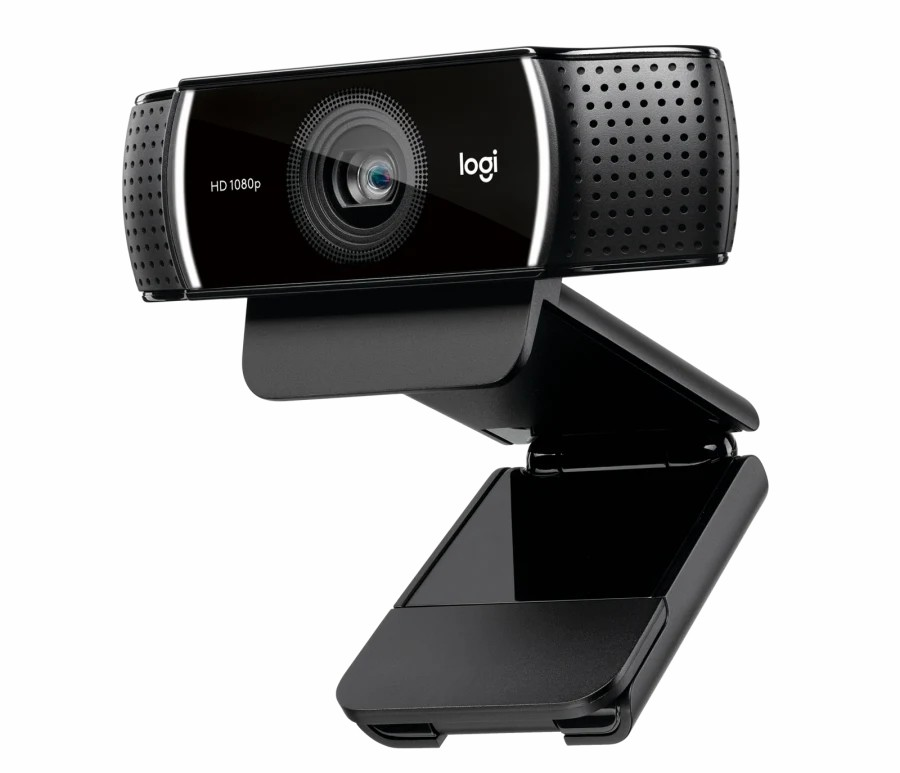
\includegraphics[width=0.7\linewidth]{figs/camera-c922.jpg}
%           \caption{Logitech c922 camera, used for testing on-site application developments}
%           \label{fig:camera-c922}
%       \end{subfigure}
%       \caption{ArUco marker used with the Logitech c922 camera for segmentation and manipulation of virtual environment}
%   \label{marker-camera}
%   \end{figure}
   commented this part because text is below - choose whether to use this or the text below

This alignment was achieved by utilizing Vuforia, a software platform that enables the creation of \ac{AR} experiences. Integrated with Unity, Vuforia simplifies the incorporation of \ac{AR} into mobile and digital apps. It uses computer vision technologies to recognize and track images and objects in the real world, allowing developers to overlay digital content precisely.

\subsection{Marker Detection}

The marker illustrated in Figure \ref{f:aruco_marker}, demonstrated greater stability, enabling the precise positioning of the digital UR10 model in alignment with the physical surroundings. Its choice followed initial attempts that yielded inconsistent results while using some other ArUco generated examples \footnote{ArUco Markers Generator \url{https://chev.me/arucogen/} Accessed: 2024-09-30}. 

To scan the physical environment around the robot, the camera shown in the figure \ref{fig:camera-c922} was used throughout the features' development process. 

\begin{figure}[h]
    \centering
    \begin{subfigure}[b]{0.45\textwidth}
    \centering
    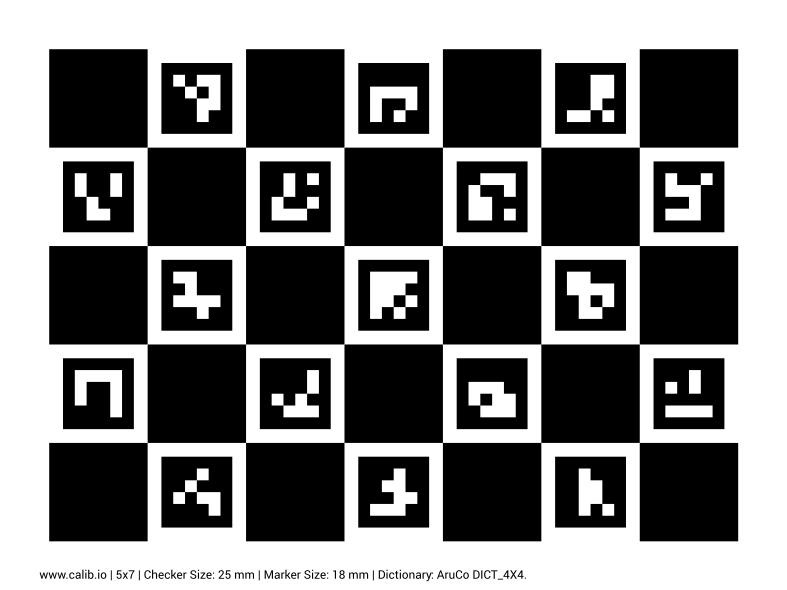
\includegraphics[width=0.7\textwidth]{figs/calib_io_charuco_200x150_5x7_25_18_DICT_4X4.png}
    \caption{ArUco marker used to allow the segmentation for aligning the digital twin accordingly to the real environment}
    \label{f:aruco_marker}
    \end{subfigure}
        \hfill % This command adds space between the subfigures
    \begin{subfigure}[b]{0.45\textwidth}
        \centering
        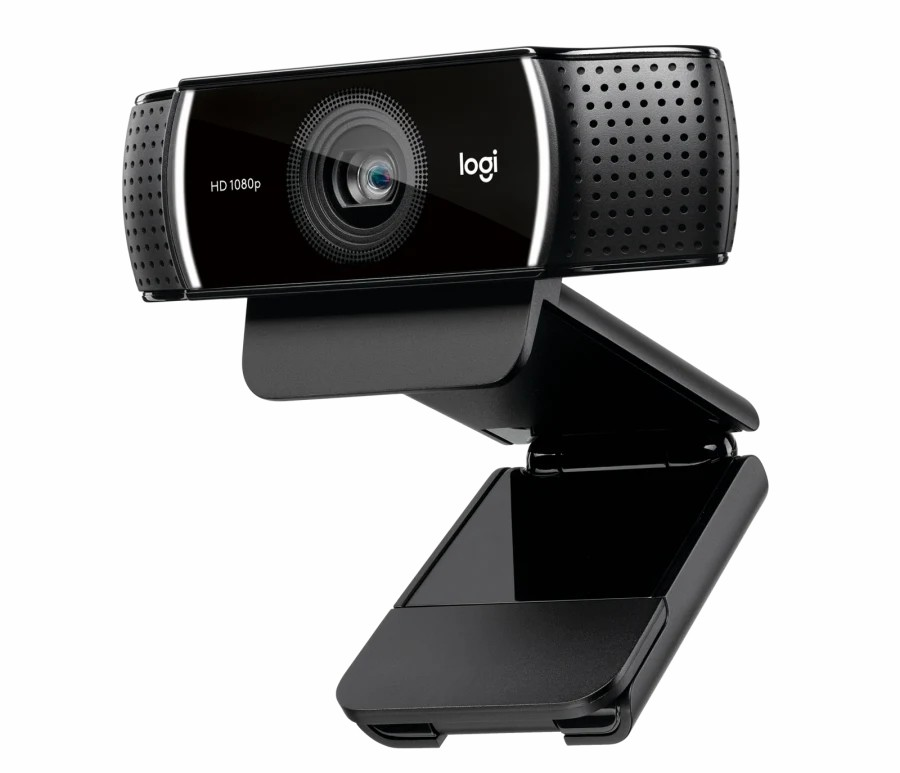
\includegraphics[width=0.7\linewidth]{figs/camera-c922.jpg}
        \caption{Logitech c922 camera, used for on-site integration}
        \label{fig:camera-c922}
    \end{subfigure}
    \caption{ArUco marker used with the Logitech c922 camera for segmentation and manipulation of virtual environment}
\label{marker-camera}
\end{figure}

Consequently, both the ArUco marker and the Logitech c922 camera allowed to overlay the digital UR10 model on top of the physical robot.
% enhancing the integration of virtual and real-world elements - use???????

In the figure \ref{f:ur10_marker_unity} it is possible to see the digital UR10 model positioned related to the aruco marker. 
    (\ref{f:aruco_marker}), in a simulated Unity environment.
    \begin{figure}[h]
    \centering
    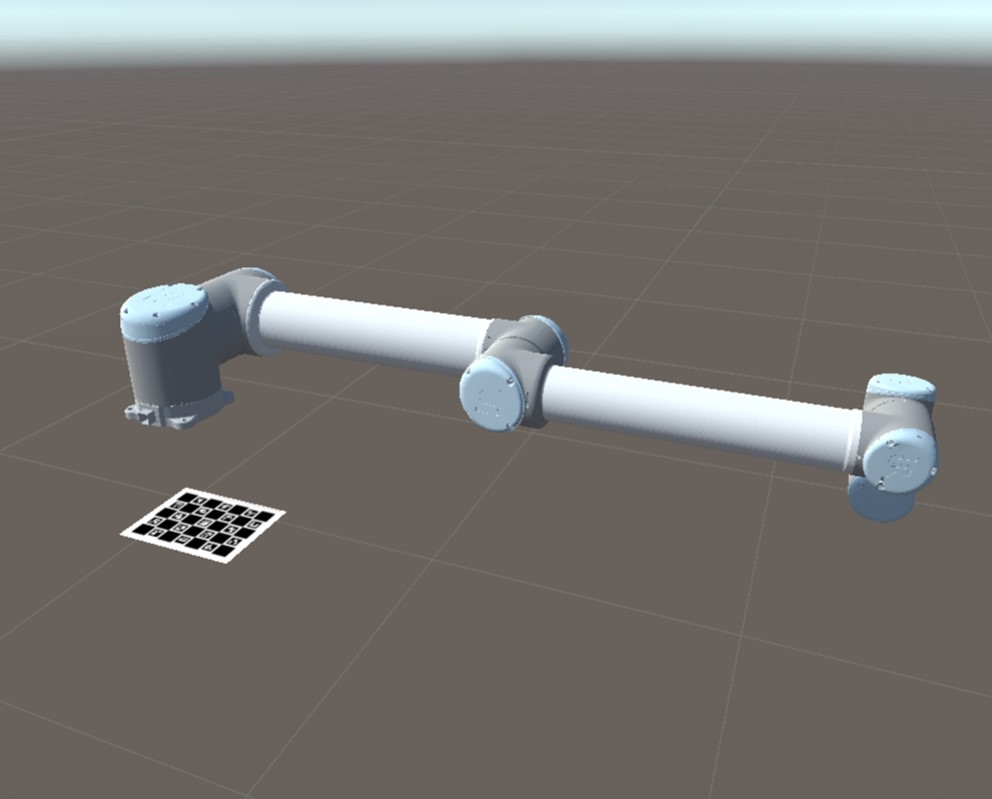
\includegraphics[width=0.6\textwidth]{figs/robot_marker_unity.jpg}
    \caption{Digital UR10 model related to the aruco marker, on Unity environment}
    \label{f:ur10_marker_unity}
    \end{figure}

\section{Billateral Communication}

\subsection{UR10e ROS Documentation}
Unity was chosen for its interactive capabilities, but this choice introduced additional complexity due to the need to operate across different operating systems—Windows for Unity and Ubuntu 20.04 for ROS Noetic, the version supporting the required ROS packages.

A key advantage was the existence of pre-existing resources from the IRIS Lab, where the robot is housed. Specifically, there were two GitHub repositories—\href{https://github.com/iris-ua/iris_sami}{iris\_sami} and \href{https://github.com/iris-ua/iris_ur10e}{iris\_ur10e}. These provided a well-established ROS environment, enabling control of the UR10e robot through RViz, trajectory planning, and real-time execution. \texttt{iris\_ur10e} package is integral to operating the physical robot in the lab, while \texttt{iris\_sami} allows for the robotic arm's manipulation.

Given this existing ROS setup on Ubuntu 20.04, ROS-TCP-Connector and ROS-TCP-Endpoint packages from the Unity Robotics Hub (\href{https://github.com/Unity-Technologies/ROS-TCP-Connector}{Unity-Technologies/ROS-TCP-Connector}) were used to establish the Wi-fi Connection. 

The proposed framework for both laptops connection is shown in figure. (add a figure of the framework proposed).


% Selecting this package over other ROS-Unity bridges was recommended by João Alves, one of the instructors who provided valuable insights during the development of this project.


\subsection{Message Generation}

By having already established the communication between Unity and ROS, specific types of messages from ROS environment had to be exchanged between the network, therefore enabling the robot to be controlled remotely.

After understanding that the ROS topic responsible for publishing the current state of the robot's joints was \texttt{/joint\_states}, these data needed to be sent to Unity. By adapting the already existing Unity Robotics Hub packages, these messages were not only successfully exchanged between the two environments, but also saved into a \texttt{.json} file for further manipulation.

\section{Robot Manipulation}
When it it came to control the digital version of the robot in the Unity environment, it was necessary to understand the Unity Robotics Hub package's way of doing so. A C\# script named \texttt{Controller.cs}, contained the necessary functions to control the robot's joints.


After further analysis, three control methods were implemented to control the robot's joints:
\begin{itemize}
    \item \textbf{UI Control:} This method allowed the user to control the \ac{DT} version of the robot by moving each joint individually through an Unity \ac{UI}. Its purpose consisted on being user-friendly and intuitive manner of controlling the robot, where a panel with a button for each joint was displayed, as shown in figure \ref{f:ui-control}. 
    
    \begin{figure}[h]
        \centering
        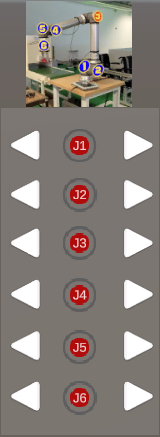
\includegraphics[width=0.6\textwidth]{figs/toggle-1.png}
        \caption{\ac{UI} panel to control the robot's joints individually}
        \label{f:ui-control}
    \end{figure}

    Besides the joints' buttons, a figure of the robot is also displayed in the top part of the panel, showing each joint's relative number, and thus allowing an easier identification of the joint to be controlled.
    
    Upon activating a joint by pressing the desired button, its color turns green instead of the default red button and the user is able to choose between rotating this joint in either the positive or negative direction, also represented by a change in the default color of the corresponding directional arrow. These features are represented in figure --- add figures joint being selected as well as the direction of UI control.
    
   
    \item \textbf{Unity-ROS Control:} This method enabled the robot to be controled during the runtime simulation in the Unity environment via the keyboard arrows of the laptop, then sending its position into the ROS environment via Wi-fi. 
    In order to change the Unity \ac{DT} robot state, the user has to press the right/left arrow keyboard keys to select the following/previous joint as well as the up/down keys to rotate the selected joint in the positive/negative direction, respectively.
    
    After updating the digital twin \ac{DT} robot's state, the user must press the "Publish" button within the user interface, shown in figure \ref{publish_UI_button}. This action publishes the current joint states over Wi-Fi to the ROS environment in a different \ac{ROS} topic than the real robot joint states are defined. 
    
    Therefore, two ROS nodes were created to handle this communication process. 
    Firstly, the \texttt{unity\_joint\_subscriber.py} was developed within the \texttt{iris\_ur10e} package, working as a subscriber to the above mentioned \ac{ROS} topic, where the \ac{DT} Unity joint states are sent to.
    Afterwards, it converts this data into a Float64MultiArray format and publishes it into yet another topic \texttt{/move\_joint\_unity} topic.
    
    Regarding the second node, the \texttt{move\_unity.py} script was created in the \texttt{iris\_sami} package. This node is a subscriber to the \texttt{/move\_joint\_unity} topic
    , which continuously listens for messages on the relevant topic. Upon receiving a new message, the ROS system updates the real robot's joint positions accordingly.

    \begin{figure}[htpb]
        \centering
        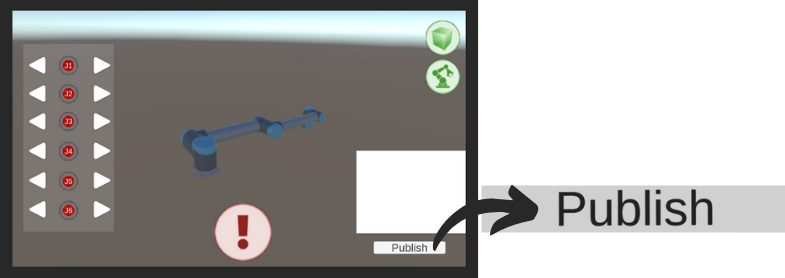
\includegraphics[width=0.7\linewidth]{figs/UI_Publish.png}
        \caption{Publish button that sends Unity's \ac{DT} robot joint states into ROS the environment}
        \label{fig:publish_UI_button}
    \end{figure}
    



    \item \textbf{Remote Control:} This method allowed the robot to be controlled remotely by using the \ac{HHD}.

\end{itemize}
Firstly a \ac{UI} was desgined to allow the on-site member to control each robot joint individually by using an 



to understand that the \texttt{Controller.cs} script was responsible for controlling the robot's joints. This script was then adapted to allow for the robot's joints to be controlled using the \ac{HHD}.




